%%%%%%%%%%%%%%%%%%%%%%%%%%%%%%%%%%%%%%%%%
% Beamer Presentation
% LaTeX Template
% Version 1.0 (10/11/12)
%
% This template has been downloaded from:
% http://www.LaTeXTemplates.com
%
% License:
% CC BY-NC-SA 3.0 (http://creativecommons.org/licenses/by-nc-sa/3.0/)
%
%%%%%%%%%%%%%%%%%%%%%%%%%%%%%%%%%%%%%%%%%

%----------------------------------------------------------------------------------------
%	PACKAGES AND THEMES
%----------------------------------------------------------------------------------------

\documentclass{beamer}

\mode<presentation>
{
  \usetheme{Madrid}      % or try Darmstadt, Madrid, Warsaw, ...
  \usecolortheme{default} % or try albatross, beaver, crane, ...
  \usefonttheme{serif}  % or try default, serif, structurebold, ...
  \setbeamertemplate{navigation symbols}{}
  \setbeamertemplate{caption}[numbered]
  \setbeamertemplate{headline}{}
}
%\usepackage[dvipsnames]{xcolor}
\usepackage[T1]{fontenc}
\usepackage[utf8]{inputenc}
\usepackage{lmodern}  
\usepackage{tikz}%boxy  
\usetikzlibrary{arrows,positioning}
\usetikzlibrary{calc}
\usepackage{amsmath}
\usepackage{bm}
\usepackage{graphicx}
\usepackage{xcolor}
\usepackage{hyperref}
%----------------------------------------------------------------------------------------
\newcommand{\mytikzmark}[2]{%
  \tikz[remember picture,inner sep=0pt,outer sep=0pt,baseline,anchor=base] 
    \node (#1) {\ensuremath{#2}};}
%
%
\newcommand*\circled[1]{\tikz[baseline=(char.base)]{
    \node[shape=circle,draw=Red,inner sep=2pt] (char) {#1};}}
%
\newcommand*\circledd[1]{\tikz[baseline=(char.base)]{
    \node[shape=circle,draw=blue, dashed, inner sep=2pt] (char) {#1};}}
%
%
\newcommand*{\boxcolor}{red}
\makeatletter
\renewcommand{\boxed}[1]{\textcolor{\boxcolor}{%
\tikz[baseline={([yshift=-1ex]current bounding box.center)}] \node [rectangle,semithick, minimum width=1ex,draw, dashed] {\normalcolor\m@th$\displaystyle#1$};}}
 \makeatother
%----------------------------------------------------------------------------------------
%	TITLE PAGE
%----------------------------------------------------------------------------------------

\title[Panel data models]{Praktikum z ekonometrie - Týden 7 \\Panel data models and tests} % The short title appears at the bottom of every slide, the full title is only on the title page

\author{VŠE Praha} % Your name
\institute[4EK417] % Your institution as it will appear on the bottom of every slide, may be shorthand to save space
{
% Your institution for the title page
\medskip
\textit{Tomáš Formánek} % Your email address
}
\date{} % Date, can be changed to a custom date

\begin{document}

\begin{frame}
\titlepage % Print the title page as the first slide
\end{frame}

\begin{frame}
\frametitle{Content} % Table of contents slide, comment this block out to remove it
\tableofcontents % Throughout your presentation, if you choose to use \section{} and \subsection{} commands, these will automatically be printed on this slide as an overview of your presentation
\end{frame}

%---------------------------------------------------------------------
%	PRESENTATION SLIDES
%---------------------------------------------------------------------
\section{Panel data models: quick repetition}
\begin{frame}{Panel data models: quick repetition}
\end{frame}
%---------------------------------------------------------------------
\begin{frame}{LSDV regression}
In the model $y_{it} = \bm{x}_{it} \bm{\beta} + \mu_i + u_{it}$, \\
\medskip
$\mu_i$ are usually regarded as unobservable variables. \\
This approach gives appropriate interpretation of $\bm{\beta}$. \\
Traditional (old) approaches to fixed effects estimation view the $\mu_i$ as parameters to be estimated along with $\bm{\beta}$. \\
\medskip
How to estimate $\mu_i$ values along with $\bm{\beta}$?
\begin{itemize}
\item Define $N$ dummy variables - one for each cross-section.
\item Convenient LSDV model expansion: use interactions to control for individual slopes for chosen regressors.
\end{itemize}
\end{frame}
%---------------------------------------------------------------------
\begin{frame}{FD estimator}
We can eliminate unobserved individual heterogeneity from the regression: \quad $y_{it} = \bm{x}_{it} \bm{\beta} + \mu_i + u_{it}$ \\
by first differences (FD) transformation: \\
$\Delta y_{it} = y_{it} - y_{i,t-1} = \Delta \bm{x}_{it} \bm{\beta} + \Delta \mu_i + \Delta u_{it} = \Delta \bm{x}_{it} \bm{\beta} + \Delta u_{it}$
\begin{itemize}
\item[$\checkmark$] Removes any unobserved heterogeneity.
\item[$\times$] We remove all time-invariant factors in $\bm{x}$.\\
If the time-invariant regressors are of no interest, this is \\a robust estimator.
\end{itemize}
Estimation can be done with FGLS (autocorrelation of transformed residuals), or OLS with HAC robust errors. \\
\medskip
FD is most suitable when we have $t = 1; 2$ – two period panel (FD may be used with more time periods, we have $N(T-1)$ observations after differencing)
\end{frame}
%---------------------------------------------------------------------
\begin{frame}{FD estimator – assumptions}
\begin{itemize}
\item[\textbf{FD.1}] Functional form: $y_{it} = \beta_1 x_{it1} + \dots + \beta_k x_{itk} + \mu_i + u_{it}$, $i = 1, \dots, N$, \ $t = 1, \dots, T$
\item[\textbf{FD.2}] We have random sample from cross-sectional units.
\item[\textbf{FD.3}] Each regressor changes in time at least for some $i$ and no perfect linear combination exists among regressors.
\item[\textbf{FD.4}] For each $i$ and $t$, \ $E (u_{it} \mid \bm{X}_i, \mu_i) = 0$. [Alt.: regressors are strictly exogenous conditional on unobserved effects: $\textit{corr}(x_{itj}, u_{is} \mid \mu_i)=0$, \quad $\forall \ t, s$]
\item[\textbf{FD.5}] Variance of differenced errors conditional on all regressors is constant: $\textit{var}(\Delta u_{it} \mid \bm{X}_i) = \sigma^2$, \quad $t= 2,3, \dots, T$. [homoskedasticity]
\item[\textbf{FD.6}] No serial correlation exists among differenced errors. $\textit{cov}(\Delta u_{it}, \Delta u_{is} \mid \bm{X}_i) = 0$, \quad $t \neq s$
\item[\textbf{FD.7}] Differenced errors are normally distributed conditional on all regressors $\bm{X}_i$.
\end{itemize}
\end{frame}
%---------------------------------
\begin{frame}{FD estimator – assumptions}
Under  \textcolor{blue}{\textbf{FD.1 - FD.4}}\\
FD estimator is unbiased. \\
FD estimator is consistent for fixed $T$ as $N \rightarrow \infty$.\\
For unbiasedness, $E (\Delta u_{it} \mid \bm{X}_i) = 0$ (for $t = 2,3, \dots$) is sufficient (instead of FD.4)\\
\medskip
Under \textcolor{blue}{\textbf{FD.1 - FD.6}}\\
FD estimator is BLUE (conditional on explanatory variables).\\
Asymptotic inference for FD estimator holds ($t$ and $F$ statistics asymptotically follow corresponding distributions).\\
\medskip
Under  \textcolor{blue}{\textbf{FD.1 - FD.7}}\\
FD estimator is BLUE (conditional on explanatory variables).\\
FD estimators - i.e. pooled OLS on first differences - are normally distributed ($t$ and $F$ statistics have exact $t$ and $F$ distributions).
\end{frame}
%---------------------------------
\begin{frame}{FD estimator}
\underline{\textbf{Problems related to the FD estimator:}}
\begin{itemize}
\item First-differenced estimates will be imprecise if explanatory variables vary only to a small extent over time (no estimate possible if regressors are time-invariant).
\item Potentially, there is insufficient (lower) variability in differenced variables.
\item Without strict exogeneity of regressors (e.g. in the case of a lagged dependent variable /say, $y_{i,t-1}$/ among regressors or with measurement errors), adding further periods does not reduce inconsistency.
\item FD estimator may be worse than pooled OLS if explanatory variables are subject to measurement errors (errors in variables - EIV).
\end{itemize}
\end{frame}
%---------------------------------------------------------------------
\begin{frame}{FE estimator}
``Fixed'' means correlation of $\mu_i$ and $\bm{x}_{it}$, not that $\mu_i$ is non-stochastic.\\ \medskip
We can rewrite $y_{it} = \bm{x}_{it} \bm{\beta} + \mu_i + u_{it}$ as follows:\\
$y_{it} = \beta_1 x_{it1} + \dots + \beta_k x_{itk} + \mu_i + u_{it},$$
\hfill $$i = 1, \dots, N$, \ $t = 1, \dots,T$ \\ 
Now, \underline{for each $i$}, we \underline{average} the above equation \underline{over time}:\\
\medskip
${\overline{y}_i = \beta_1 \overline{x}_{i1} + \dots + \beta_k \overline{x}_{ik} + \overline{\mu}_i + \overline{u}_i}$\\ ($N$ equations with individual averages)
\medskip
By subtracting individual averages from the original observations (time-demeaning), we get:\\
$\Rightarrow \boxed{[y_{it} - \overline{y}_{i}]} = \beta_1 \boxed{[x_{it1}-\overline{x}_{i1}]}+\dots+\beta_k \boxed{[x_{itk}-\overline{x}_{ik}]}+\boxed{[u_{it}- \overline{u}_i]}$\\
\medskip
Alternative notation: $\ddot{y}_{it} = \bm{\ddot{x}}_{it} \bm{\beta} + \ddot{u}_{it}$; where $\ddot{y}_{it} = y_{it} - \overline{y}_{i}$, etc.\\
\medskip
FE estimator, denoted $\bm{\hat{\beta}}_{FE}$, is the pooled OLS estimator applied to time-demeaned data.
\end{frame}
%---------------------------------------------------------------------
\begin{frame}{FE estimator}
\textbf{FE estimator:} by time demeaning, we get rid of the $\mu_i$ element - as it does not vary over time 
\vspace{0.5cm}
\begin{itemize}
\item $\mu_i = \overline{\mu}_i \ \rightarrow \ \mu_i - \overline{\mu}_i = 0$
\item Intercept and all time-invariant regressors are also eliminated using the FE (within) transformation.
\end{itemize}
\vspace{0.5cm}
After FE estimation, $\mu_i$ elements may be estimated as follows:
$\hat{\mu}_i =\overline{y}_i - \hat{\beta}_1 \overline{x}_{i1} - \dots - \hat{\beta}_k \overline{x}_{ik},$ \ $i = 1, \dots, N$ \\
\vspace{0.5cm}
However, in most practical applications, $\mu_i$ values bear limited useful information.\\ \medskip
For each C-S observation $i$, we loose one d.f. in estimation ~ \dots for each $i$, the demeaned errors $\ddot{u}_{it}$ add up to zero when summed over time. Hence \ $df = N(T-1)-k$
\end{frame}
%---------------------------------------------------------------------
\begin{frame}{FE estimator – assumptions}
\begin{itemize}
\item[\textbf{FE.1}] Functional form: $y_{it} = \beta_1 x_{it1} + \dots + \beta_k x_{itk} + \mu_i + u_{it}$, $i = 1, \dots, N$, \ $t = 1, \dots, T$
\item[\textbf{FE.2}] We have random sample from cross-sectional units.
\item[\textbf{FE.3}] Each regressor changes in time at least for some $i$ and no perfect linear combination exists among regressors.
\item[\textbf{FE.4}] For each $i$ and $t$, \ $E (u_{it} \mid \bm{X}_i, \mu_i) = 0$. [Alt.: regressors are strictly exogenous conditional on unobserved effects: $\textit{corr}(x_{itj}, u_{is} \mid \mu_i)=0$, \quad $\forall \ t, s$]
\item[\textbf{FE.5}] Variance of errors conditional on all regressors is constant: $\textit{var}(u_{it} \mid \bm{X}_i, \mu_i) = \textit{var}(u_{it}) = \sigma^2_u$, \quad $t= 1,2, \dots, T$. [homoskedasticity]
\item[\textbf{FE.6}] No serial correlation exists among idiosyncratic errors. $\textit{cov}(u_{it}, u_{is} \mid \bm{X}_i, \mu_i) = 0$, \quad $t \neq s$
\item[\textbf{FE.7}] Errors are normally distributed conditional on all regressors $(\bm{X}_i, \mu_i)$.
\end{itemize}
\end{frame}
%---------------------------------
\begin{frame}{FE estimator – assumptions}
Under \textcolor{blue}{\textbf{FE.1 - FE.4}} (identical to  \textcolor{blue}{\textbf{FD.1 - FD.4}})\\
FE estimator is unbiased. \\
FE estimator is consistent for fixed $T$ as $N \rightarrow \infty$.\\
\vspace{0.5cm}
Under \textcolor{blue}{\textbf{FE.1 - FE.6}}\\
FE estimator is BLUE.\\
FD is unbiased\\ \dots  \textcolor{blue}{\textbf{FE.6}} makes FE better (less variance) than FD.\\
Asymptotically valid inference for FE estimator holds ($t$ and $F$).\\
\vspace{0.5cm}
Under  \textcolor{blue}{\textbf{FE.1 - FE.7}}\\
FE estimator is BLUE and $t$ and $F$ statistics have exact $t$ and $F$ distributions.\\
FE estimators - i.e. pooled OLS on time demeaned data - are normally distributed.
\end{frame}
%---------------------------------
\begin{frame}{FE vs FD estimator}
\begin{itemize}
\item For $T=2$, FE and FD estimators produce identical estimates and inference. (FE must include a time dummy for the second period to be actually identical to the FD estimation output)
\item For $T>2$, FE and FD are both unbiased under FE.1 - FE.4. Both FE and FD are consistent for fixed $T$ as $N \rightarrow \infty$
\item If $u_{it}$ is not serially correlated, FE is more efficient than FD
\item If $u_{it}$ follows a random walk (hence $\Delta u_{it}$ is serially uncorrelated) FD is better than FE.
\item If $u_{it}$ shows some level of positive serial correlation (not a random walk), FD and FE may not be easily compared. For negative correlation of $u_{it}$, we prefer FE.
\end{itemize}
\end{frame}
%---------------------------------
%\begin{frame}{FE vs FD estimator}
%\begin{itemize}
%\item For $T \gg N$, especially if non-stationary series are involved, FE may lead to spurious regression problems, while the FD help us transforming integrated series into weakly dependent series.
%\item If strict exogeneity is violated, both FE and FD are biased. However, FE is likely to have less bias than FD (unless $T=2$). The bias of FD does not depend on $T$, while the bias in FE tends to zero at rate $1/T$.
%\item \dots it may be a good idea to use both FD and FE. If the results are not method-sensitive, so much the better. If the results from FE and FD differ significantly, we sometimes report both.
%\end{itemize}
%\end{frame}
%---------------------------------
\begin{frame}{RE estimator}
If $\mu_i$ are uncorrelated with $\bm{x}_{it}$, then it may be appropriate to model the individual constant terms as randomly distributed across cross-sectional units (appropriate if C-S units are from a large sample).
\bigskip

\begin{itemize}
\item RE models reduce the number of parameters estimated.
\item RE estimator is potentially inconsistent, if assumption not met.
\item $y_{it} = \bm{x}_{it} \bm{\beta} + \mu_i + u_{it}$\\
\item If we can assume that $\mu_i$ is uncorrelated with each explanatory variable: $\textit{cov}(\bm{x}_{it}, \mu_i) = 0$; \ $t = 1,2, \dots, T$ \\then we may drop $\mu_i$ from the equation and $\beta_j$ estimates will remain unbiased.\\
\item By dropping $\mu_i$ from the regression, we effectively create a new error term: $v_{it} = \mu_i + u_{it}$\\
\medskip
\item As $\mu_i$ is time-invariant, the random element $v_{it}$ contains a lot of ``inertia'', i.e. autocorrelation (unless $\mu_i = 0$).
\end{itemize}
\end{frame}
%---------------------------------
\begin{frame}{RE estimator - FGLS}
$y_{it} = \beta_0 + \beta_1 x_{it1} + \dots + \beta_k x_{itk} + v_{it};$\\
%\bigskip
The quasi-demeaning (quasi-differencing) parameter $\lambda$ is used for the FGLS estimation:\\
$\theta = 1 - \big[ \sigma^2_u / (\sigma^2_u + T \sigma^2_{\mu}) \big]^{1/2}$, \quad  $0 \le \theta \le 1$\\
%\medskip
where $\textit{var}(\mu_i) = \sigma^2_{\mu}$; \quad $\textit{var}(u_i) = \sigma^2_u$\\
\begin{itemize}
\item \small For each dataset, consistent estimators of $\sigma^2_{\mu}$ and $\sigma^2_u$ are available.\\
\item \small Their estimation is based on pooled OLS or FE \\ also, we use the fact that $\sigma^2_v = \sigma^2_{\mu} + \sigma^2_u$\\
\end{itemize}
%\medskip
\vspace{-0.1cm}
RE estimator is a pooled OLS used on the quasi-demeaned data:\\
\vspace{-0.3cm}
\small $$\boxed{[y_{it} - \theta \overline{y}_i]} = \beta_1  \boxed{[x_{it1}- \theta \overline{x}_{i1}]}+\dots+\beta_k \boxed{[x_{itk}- \theta \overline{x}_{ik}]}+ \boxed{[\mu_i - \theta \overline{a}_i + u_{it}-\theta \overline{u}_i]}$$
(transformed errors follow G-M assumptions -- not autocorrelated)
\end{frame}
%---------------------------------
\begin{frame}{RE estimator - FGLS}
\
{\footnotesize $$\boxed{[y_{it} - \theta \overline{y}_i]} = \beta_1 \boxed{[x_{it1}- \theta \overline{x}_{i1}]}+\dots+\beta_k \boxed{[x_{itk}- \theta \overline{x}_{ik}]}+\boxed{[\mu_i - \theta \overline{a}_i + u_{it}-\theta \overline{u}_i]}$$}\\
\bigskip
Interestingly, the FGLS equation is a general form that encompasses both FE and pooled OLS:
\bigskip
\begin{align*}
\hat{\theta} \rightarrow 1 \quad & \rightarrow \quad \textnormal{RE}  \rightarrow \ \textnormal{FE}\\
\hat{\theta} \rightarrow 0 \quad & \rightarrow \quad \textnormal{RE}  \rightarrow \ \textnormal{Pooled}
\end{align*}
\end{frame}
%---------------------------------
\begin{frame}{RE estimator – Assumptions}
\footnotesize
\begin{itemize}
\item[\textbf{FE.1}] Functional form: $y_{it} = \beta_1 x_{it1} + \dots + \beta_k x_{itk} + \mu_i + u_{it}$, $i = 1, \dots, N$, \ $t = 1, \dots, T$
\item[\textbf{FE.2}] We have random sample from cross-sectional units.
\item[\textbf{FE.4}] $\forall \ i, t$: \ $E (u_{it} \mid \bm{X}_i, \mu_i) = 0$. [Alt.: $\textit{corr}(x_{itj}, u_{is} \mid \mu_i)=0$, \ $\forall \ t, s$]
\item[\textbf{FE.5}] Variance of idiosyncratic errors conditional on all regressors is constant: $\textit{var}(u_{it} \mid \bm{X}_i, \mu_i) = \textit{var}(u_{it}) = \sigma^2_u$, \quad $t= 1,2, \dots, T$. [homoskedasticity]
\item[\textbf{FE.6}] No serial correlation exists among idiosyncratic errors. $\textit{cov}(u_{it}, u_{is} \mid \bm{X}_i, \mu_i) = 0$, \quad $t \neq s$
\item[\textcolor{black}{\textbf{FE.7}}] [normality of $u_{it}$ has little actual importance for the RE estimator
\end{itemize}
	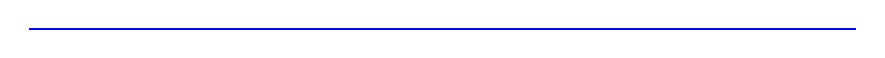
\begin{tikzpicture}
	\draw[thick, color=blue] (0,0) -- (10.5,0);
	\end{tikzpicture}
\begin{itemize}
\item[\textbf{RE.1}] There are no perfect linear relationships among explanatory variables. [replaces \textcolor{blue}{\textbf{FE.3}}]
\item[\textbf{RE.2}] In addition to \textcolor{blue}{\textbf{FE.4}}, the expected value of $\mu_i$ given all regressors is constant: $E(\mu_i \mid \bm{X}_i)=\beta_0$. [Rules out correlation between $\mu_i$ and $\bm{X}_i$]
\item[\textbf{RE.3}] In addition to \textcolor{blue}{\textbf{FE.5}}, variance of $\mu_i$ given all regressors is constant: $\textit{var}(\mu_i \mid \bm{X}_i)=\sigma^2_a$ [Homoskedasticity imposed on $\mu_i$]
\end{itemize}
\end{frame}
%---------------------------------
\begin{frame}{RE estimator – Assumptions}
Under  \textcolor{blue}{\textbf{FE.1+FE.2+RE.1+(FE.4+RE.2)}}\\
RE estimator is consistent and asymptotically normal \\(for fixed $T$ as $N \rightarrow \infty$).\\
RE standard errors and statistics are not valid unless \textcolor{blue}{\textbf{(FE.5+RE.3)}} and  \textcolor{blue}{\textbf{FE.6}} conditions are met.\\
\bigskip
Under  \textcolor{blue}{\textbf{FE.1-FE.2+RE.1+(FE.4+RE.2)+(FE.5+RE.3)+FE.6}}\\
RE estimator is consistent and asymptotically normal \\(for fixed $T$ as $N \rightarrow \infty$).\\
RE standard errors and statistics are valid.\\
RE is asymptotically efficient 
\begin{itemize}
\item[-] lower st.errs. than pooled OLS
\item[-] for time-varying variables, RE estimator is more efficient than FE (FE cannot be used on time-invariant variables).
\end{itemize}
\end{frame}
%---------------------------------
\begin{frame}{CRE estimator}
Correlated Random Effects (CRE) estimator - a synthesis of the RE and FE approaches: 
\vspace{0.5cm}
\begin{itemize}
\item $\mu_i$ viewed as random, yet they can be correlated with $\bm{x}_{it}$.\\
\vspace{0.2cm}
Specifically, as $\mu_i$ do not vary over time, it makes sense to allow for their correlation with the time average of $x_{it}:\overline{x}_i = T^{-1} \sum^T_{t=1}x_{it}$
\vspace{0.2cm}
\item CRE allows for incorporation of time-invariant regressors (compare to FE).
\vspace{0.2cm}
\item CRE allows for convenient testing of FE vs. RE.
\end{itemize}
\end{frame}
%---------------------------------
\begin{frame}{CRE estimator}
CRE: The individual-specific effect $\mu_i$ is split up into a part that is related to the time-averages of the explanatory variables and a part $r_i$ (a time-constant unobservable) that is unrelated to the explanatory variables: 
\begin{align*}
\textnormal{For } y_{it} & =  \beta_1 x_{it} + \mu_i + u_{it}\textnormal{, we assume (a single-regressor illustration):}\\ \vspace{0.3cm}
\mu_i & = \alpha + \gamma \overline{x}_i + r_i \textnormal{, now: } \textit{cor}(r_i, \overline{x}_i) = 0 \Rightarrow \textit{cor}(r_i,x_{it}) = 0\\ 
&\textnormal{~~(because $\overline{x}_i$  is a linear function of  $x_{it}$)}
\end{align*}

By substituting for $\mu_i$ into the first equation, we obtain: \\
$y_{it} = \alpha + \beta_1 x_{it} + \gamma \overline{x}_i + r_i + u_{it}$ \\
\bigskip
\underline{This equation can be estimated using RE}\\
As $\gamma \overline{x}_i$ controls for the correlation between $\mu_i$ and $x_{it}$, \\$r_i$ is uncorrelated with regressors.
\end{frame}
%---------------------------------
\begin{frame}{CRE estimator}
CRE: \ $y_{it} = \alpha + \beta_1 x_{it} + \gamma \overline{x}_i + r_i + u_{it}$ \\
\medskip
\small CRE is a modified RE of the original equation $y_{it} =  \beta_1 x_{it} + \mu_i + u_{it}$: \\
\vspace{0.2cm}
with uncorrelated random effect $r_i$ but with the time averages as additional regressors. \\
\vspace{0.3cm}
\underline{The resulting CRE estimate for $\beta$ is identical to the FE estimator}.
\begin{itemize}
\item CRE allows for incorporation of time-invariant regressors: Besides $\hat{\beta}_{\textit{CRE}} = \hat{\beta}_{\textit{FE}}$, we can include arbitrary time invariant regressors and estimate $\gamma_{\textit{CRE}}$ values.
\item CRE allows for convenient testing of FE vs. RE:
	\begin{itemize}
	\item[$H_0$:] $\gamma = 0$ can be evaluated using $\hat{\gamma}_{\textit{CRE}}$ and appropriate (HCE) standard errors against
	\item[$H_1$:] $\gamma \neq 0$
	\end{itemize}
\end{itemize}
[RE assumes $\gamma = 0$: if we reject $H_0$, we also reject RE in favor of FE]
\end{frame}
%---------------------------------
\begin{frame}{Arellano-Bond estimator (dynamic panels)}
Dynamic panel\\
\medskip
$y_{it} = \delta_1 y_{i,t-1} + \bm{x}^{\prime}_{it} \bm{\beta} + \mu_i + u_{it}$\\
\medskip
\dots May be expanded using additional lags of the dependent variable or using lagged exogenous regressors.\\
\medskip
\small
\textbf{Nickel Bias}
\begin{itemize}
\item Related mostly to the lagged exogenous regressors $\bm{x}$
\item FEs take up some part of the dynamic effect and therefore dynamic panel data models lead to overestimated FEs and underestimated dynamic interactions. 
\item Whether the Nickel bias is significant in a particular model/dataset situation is an empirical question. Nevertheless, in theory this bias persists unless the number of time observations goes to infinity.
\item The inclusion of additional cross-sections to the dataset would worsen the bias in most cases.
\end{itemize}
\end{frame}
%---------------------------------
\begin{frame}{Arellano-Bond estimator (dynamic panels)}
\textbf{Arellano-Bond} (AB) \textbf{estimator} 
\begin{itemize}
\item The model is transformed into first differences to eliminate the individual effects:\\
$\Delta y_{it} = \delta_1 \Delta y_{i,t-1} + \Delta \bm{x}^{\prime}_{it} \bm{\beta} + \Delta u_{it}$, 
\item then a generalized method of moments (GMM) approach is used to produce asymptotically efficient estimates for the dynamic coefficients.
\item AB approach is based on IV (we need instruments for the lagged dependent variable – this is an endogenous regressor, correlated with the errors in the FD model).
\item \textcolor{red}{Warning:} AR(2) / not AR(1) / autocorrelation in residuals of the AB-estimated model renders the AB estimator inconsistent. After using the AB estimator, always test for AR(2) autocorrelation in the residuals!
\end{itemize}
\end{frame}
%---------------------------------------------------------------------
\section{Poolability tests}
\begin{frame}{Poolability tests}
\end{frame}
%---------------------------------------------------------------------
\begin{frame}{LSDV-based test for individual intercepts}
\begin{itemize}
    \item Null hypothesis of common intercept is tested against the alternative of individual-specific intercepts.
    \medskip
    \item Common slopes are assumed (not tested)
    \medskip
    \item Unrestricted model: $y_{it} = \beta_{0} + \bm{d}^{\prime}\bm{\delta}_{0} + \beta_1 x_{it1} + \beta_2 x_{it2} + u_{it}$ \\ 
    where $\bm{d}$ is a vector of CSID-based dummy variables and $\bm{\delta}_{0}$ is a vector of regression coefficients ($N-1$ dummies used to avoid dummy variable trap).
    \medskip
    \item Restricted model: $~~y_{it} = \beta_{0}~ \, + \beta_1 x_{it1} + \beta_2 x_{it2} + u_{it}$.
    \medskip
    \item Can be implemented as an $F$-test for linear (zero) restrictions: Pooled regression vs LSDV model
\end{itemize}
\end{frame}
%---------------------------------------------------------------------
\begin{frame}{Chow test for identical slopes}
\begin{itemize}
    \item \texttt{pooltest()} from the \texttt{\{plm\}} package 
    \smallskip
    \item We allow for different intercepts \& test for equal slopes \\in all CS-units
    \begin{itemize}
        \item Estimate model separately for each CS unit.
        \item Compare with ``FE'' model (individual intercept, common slopes on regressors) using an $F$-test -- are the slopes identical among CS-units?
    \end{itemize}
    \smallskip
    \item Drawback: test cannot handle time-invariant regressors (FE; also, as the unrestricted model is estimated individually for each CS-unit, such regressors are perfectly correlated with the intercept and $\mu_i$ elements)
    \medskip
    \item Unrestricted model: $y_{it} = \beta_{0} + \beta_{i1} x_{it} + \mu_i + u_{it}$
    \smallskip
    \item Restricted model: $\,~~y_{it} = \beta_{0}~ \, + \beta_1 x_{it} + \mu_i + u_{it}$
\begin{itemize}
    \item[] $H_0:~\beta_{11}=\beta_{21}=\dots=\beta_{N1}$  
    \item[] $H_1:~\neg H_0$
\end{itemize}
\end{itemize}
\end{frame}
%---------------------------------------------------------------------
\begin{frame}{Chow test for identical slopes}
\vspace{2.5cm}
\vfill
\bigskip
$F=\frac{ \mytikzmark{SSRr}{\textit{SSR}_r}- \mytikzmark{SSRur}{\textit{SSR}_{ur}}}{\textit{SSR}_{ur}} \cdot \frac{(NT-N-Nk)}{(N-1)k};$ \\
\bigskip
{\small under $H_0$ of no structural break, $F \sim F[(N-1)k, (NT- \mytikzmark{TTk}{\circledd{$N-Nk$)}}]$} \\
\bigskip
\begin{itemize}
\item Alternatively, the restricted model can be amended to feature \\a single intercept (no $\mu_i$ individual effects).
\end{itemize}
\begin{tikzpicture}[<-,overlay,remember picture,inner sep=1.5pt,shorten <=0.2em,font=\scriptsize]
\tikzset{
    mynode/.style={rectangle,draw=blue, dashed, fill=white, semithick, inner sep=.2em, minimum size=2em, text centered, text width=9em},
    myarrow/.style={->, >=stealth, thin, blue}
}
\node[mynode] at (1.8,7.2) (SSRr*){$\textit{SSR}_r$: restricted model – allow for different $\mu_i$, impute common slopes.};
\draw[myarrow] (SSRr*) -- ++   (SSRr);
	\node[mynode] at (5.5,7.2) (SSRur*){$\textit{SSR}_{ur}$:run a regression for each of the CS units. $\textit{SSR}_{ur} = 			\textit{SSR}_1 + \textit{SSR}_2 + \dots + \textit{SSR}_N$};
	\draw[myarrow] (SSRur*) -- ++   (SSRur);
		\node[mynode] at (9.3,7.2) (TTk*){$N + Nk$ parameters estimated in the unrestricted model, $k$ is \# regressors};
		\draw[myarrow] (TTk*) -- ++   (TTk);
\end{tikzpicture}
\end{frame}
%---------------------------------------------------------------------
\begin{frame}{Honda (1985) test for individual and time effects}
\begin{itemize}
    \item \texttt{plmtest(..., type="honda")} from the \texttt{\{plm\}} package
    \medskip
    \item Using OLS-based (``pooling'') residuals, we test the null hypothesis of redundant individual $(\mu_i)$ and/or time $ (\lambda_t) $ effects.
    \medskip
    \item Individual effects: 
    $$y_{it} = \beta_{0} + \beta_{1} x_{it1} + \dots + \beta_k x_{itk} + \mu_i + \nu_{it}$$
    \item Time effects: 
    $$y_{it} = \beta_{0} + \beta_{1} x_{it1} + \dots + \beta_k x_{itk} + \lambda_t + \nu_{it}$$  
    \item Twoways effects: 
    $$~~~~~y_{it} = \beta_{0} + \beta_{1} x_{it1} + \dots + \beta_k x_{itk} + \mu_i + \lambda_t + \nu_{it}$$ \item Note: for this LM-based tests, we only use the residuals of the pooling model (if performed on RE of FE model, corresponding pooling model is calculated internally first). \\ \smallskip Notation follows Baltagi (2008)
\end{itemize}
\end{frame}
%---------------------------------------------------------------------
\begin{frame}{Honda (1985) test for individual and time effects}
Panel model\\ \bigskip
\begin{itemize}
    \item $y_{it} = \alpha + \bm{x}^{\prime}_{it} \bm{\beta} + u_{it} \qquad$    where $u_{it}=\mu_i + \lambda_t + \nu_{it}$
    \medskip
    \item Assumptions for Honda (1985) test: \\ \smallskip {\it i.i.d.} individual effects: $\mu_i \sim N(0,\sigma^2_{\mu})$; \\{\it i.i.d.} time effects: $\lambda_t \sim N(0,\sigma^2_{\lambda})$; \\{\it i.i.d.} idiosyncratic errors: $\nu_{it} \sim N(0,\sigma^2_{\nu})$.
    \medskip
    \item Null hypotheses to be tested:
    \smallskip
    \begin{itemize}
        \item $H_0^{\mu}: \sigma^2_{\mu} = 0 \qquad \qquad$ ~~~(no individual effects)
        \smallskip
        \item $H_0^{\lambda}: \sigma^2_{\lambda} = 0 \qquad \qquad$ ~~~(no time effects)
        \smallskip
        \item $H_0^{\mu \lambda}: \sigma^2_{\mu} = \sigma^2_{\lambda} = 0 \qquad \,$ (no individual nor time effects)
    \end{itemize}
\end{itemize}
\end{frame}
%---------------------------------------------------------------------
\begin{frame}{Honda (1985) test for individual and time effects}
$y_{it} = \alpha + \bm{x}^{\prime}_{it} \bm{\beta} + u_{it} \qquad$    where $u_{it}=\mu_i + \lambda_t + \nu_{it}$\\ \smallskip Balanced panel assumed. \bigskip
\begin{itemize}
    \item Error component in stacked (matrix form): \\ \smallskip
    $\bm{u}_i = \left( u_{i1}, u_{i2}, \dots, u_{iT} \right)^{\prime}$ and $\bm{u} = \left( \bm{u}_1^{\prime}, \bm{u}_2^{\prime}, \dots, \bm{u}_N^{\prime} \right)^{\prime}$ \\ \smallskip
    $\bm{u}_i$ is $T \times 1$ and $\bm{u}$ is $NT \times 1$.
    \medskip
    \item In matrix form, $\bm{u}$ can be cast as: \\
    $\bm{u} = \bm{D}_{\mu} \bm{\mu} + \bm{D}_{\lambda} \bm{\lambda} + \bm{\nu}$ \\ \smallskip
    where \\$\bm{\mu} = (\mu_1, \dots, \mu_N)^{\prime}$, \\$\bm{\lambda} = (\lambda_1, \dots, \lambda_T)^{\prime}$, \\$\bm{\nu}$ follows the structure of $\bm{u}$,\\
    $\bm{D}_{\mu} = (\bm{I}_N \otimes \bm{\iota}_T)$ i.e. $\bm{I}_N$ with each row repated $T$-times; $(NT \times N)$, \\
    $\bm{D}_{\lambda} = ( \bm{\iota}_N \otimes \bm{I}_T )$ i.e. $\bm{I}_T$ stacked vertically $N$-times; $(NT \times T)$, \\ 
    note that time is the ``fast index'' here.
    \end{itemize}
\end{frame}
%---------------------------------------------------------------------
\begin{frame}{Honda (1985) test for individual and time effects}
$y_{it} = \alpha + \bm{x}^{\prime}_{it} \bm{\beta} + u_{it} \qquad$    where $u_{it}=\mu_i + \lambda_t + \nu_{it}$\\ \medskip
$\bm{u} = \bm{D}_{\mu} \bm{\mu} + \bm{D}_{\lambda} \bm{\lambda} + \bm{\nu}$ \\ \bigskip
\begin{itemize}
    \item $\bm{D}_{\mu} \bm{D}_{\mu}^{\prime} = \left(\bm{I}_N \otimes \bm{J}_T \right)$ i.e. block-diagonal matrix of $\bm{J}_T$-matrices \\where $\bm{J}_T=\iota_T \iota_T^{\prime}$  ($\bm{J}_T$ is a $T \times T$ matrix of ones).
    \medskip
    \item $\bm{D}_{\lambda} \bm{D}_{\lambda}^{\prime} = \left(\bm{J}_N \otimes \bm{I}_T   \right)$ i.e. $N\times N$ array of $\bm{I}_T$-matrices.
    \medskip
    \item Now, we define\\ \medskip
    $A_r = \left[ \left( \frac{\bm{u}^{\prime}\bm{D}_r \bm{D}_r^{\prime} \bm{u}}{\bm{u}^{\prime}\bm{u}} \right) - 1 \right]$ for $r=\mu$ or $r=\lambda$.
    \end{itemize}
\end{frame}
%---------------------------------------------------------------------
\begin{frame}{Honda (1985) test for individual and time effects}
$y_{it} = \alpha + \bm{x}^{\prime}_{it} \bm{\beta} + u_{it} \qquad$    where $u_{it}=\mu_i + \lambda_t + \nu_{it} \qquad$ (balanced panel)\\ \medskip
\begin{itemize}
    \item Honda (1985) derives a uniformly most powerful {\it LM} statistics for \\
    $H_0^{\mu}: \sigma_{\mu}^2=0$ against a one-sided $H_1^{\mu}: \sigma_{\mu}^2>0$:
    $$
    \textnormal{HO}_{\mu} = \sqrt{\frac{NT}{2(T-1)}} ~ A_{\mu} ~ \underset{H_0}{\rightarrow}~N(0,1)
    $$
    \item Similarly, for $H_0^{\lambda}: \sigma_{\lambda}^2=0$ against a one-sided $H_1^{\lambda}: \sigma_{\lambda}^2>0$:
    $$
    \textnormal{HO}_{\lambda} = \sqrt{\frac{NT}{2(T-1)}} ~ A_{\lambda} ~ \underset{H_0}{\rightarrow}~N(0,1)
    $$
\end{itemize}    
\end{frame}
%---------------------------------------------------------------------
\begin{frame}{Honda (1985) test for individual and time effects}
$y_{it} = \alpha + \bm{x}^{\prime}_{it} \bm{\beta} + u_{it} \qquad$    where $u_{it}=\mu_i + \lambda_t + \nu_{it} \qquad$ (balanced panel)\\ \medskip
\begin{itemize}
    \item Honda (1985) provides a test statistic for $H_0^{\mu \lambda}: \sigma_{\mu}^2=\sigma_{\lambda}^2=0$ against a one-sided alternative
    \\(not derived as a uniformly most powerful {\it LM} statistics):
    $$
    \textnormal{HO}_{\mu \lambda} = \frac{\textnormal{HO}_{\mu}+\textnormal{HO}_{\lambda}}{\sqrt{2}} {\rightarrow}~N(0,1)
    $$
    \bigskip
    \item Honda (1985) statistics can be generalized to the unbalanced case. \\see e.g.: \footnotesize{\textcolor{blue}{\underline{http://www.eviews.com/help/}}}
\end{itemize}    
\end{frame}
%---------------------------------------------------------------------
\begin{frame}{$F$-test for unobserved effects (FE-based) vs pooling model}
$y_{it} = \alpha + \bm{x}^{\prime}_{it} \bm{\beta} + \mu_i + \lambda_t + \nu_{it}$\\ \medskip
\begin{itemize}
    \item \texttt{pFtest()} from the \texttt{\{plm\}} package
    \medskip
    \item $F$-test of effects based on the comparison of ``pooling'' and ``within'' models (either ``individual'', ``time'' or ``twoways'' effects can be tested).
    \medskip
    \item Hence, two main arguments to the test function are \texttt{plm}-estimated ``pooling'' and ``within'' models. 
    \medskip 
    \item d.f. of the $F$-test depend on the number of observations and parameters restricted:\\
    \texttt{df1} is the number of parameters restricted, \\
    \texttt{df2} $= N(T-1)~-$ (\# parameters est. in the unrestricted model)    \dots remember that for each C-S observation $i$, we loose one d.f. as the demeaned errors $\ddot{\nu}_{it}$ add up to zero when summed over time.
\end{itemize}    
\end{frame}
%---------------------------------------------------------------------
\section{Estimator selection \& serial correlation tests}
\begin{frame}{Estimator selection \& serial correlation tests}
\end{frame}
%---------------------------------------------------------------------
\begin{frame}{Hausman test: RE vs FE estimator}
\begin{itemize}
    \item \texttt{phtest()} from the \texttt{\{plm\}} package
    \medskip
    \item Hausman test is based on the comparison of two sets of estimates
    \medskip
    \item A classical application of the Hausman test for panel data is to compare the fixed and the random effects models:
    {\small $$H=(\hat{\bm{\beta}}_{FE} - \hat{\bm{\beta}}_{RE})^T [\widehat{\textit{Avar}}(\hat{\bm{\beta}}_{FE}) - \widehat{\textit{Avar}}(\hat{\bm{\beta}}_{RE})]^{-1} (\hat{\bm{\beta}}_{FE} - \hat{\bm{\beta}}_{RE}) \underset{H_0}{\sim} \chi^2(m)$$}
    {\footnotesize where $m$ is the number of regressors varying across $i$ and $t$.}
    \smallskip
    \item[] $H_0$: $\textnormal{cov}(\bm{x}_{it},\mu_i) = 0$ \dots i.e. the crucial RE assumption holds
    \item[] $H_1$: RE assumptions violated.
\end{itemize}
\end{frame}
%---------------------------------
\begin{frame}{Hausman test: RE vs FE estimator}

{\small $$H=(\hat{\bm{\beta}}_{FE} - \hat{\bm{\beta}}_{RE})^T [\widehat{\textit{Avar}}(\hat{\bm{\beta}}_{FE}) - \widehat{\textit{Avar}}(\hat{\bm{\beta}}_{RE})]^{-1} (\hat{\bm{\beta}}_{FE} - \hat{\bm{\beta}}_{RE}) \underset{H_0}{\sim} \chi^2(m)$$}
\medskip
\begin{itemize}
    \item If $\hat{\bm{\beta}}_{FE}$ and $\hat{\bm{\beta}}_{RE}$ do not differ too much [or when the asymptotic variances are relatively large] we do not reject $H_0$. 
    \medskip
    \item If we may assume RE assumptions hold, both RE and FE are consistent, and RE is efficient. 
    \medskip
    \item For asymptotic variance estimators ($\widehat{\textit{Avar}}$), see Wooldridge (2010). 
    \medskip
    \item If we reject $H_0$, we need to assume that RE assumptions are violated $\rightarrow$ RE is not consistent [we use FE].
\end{itemize}
\end{frame}
%---------------------------------
\begin{frame}{Wooldridge's FD-based test: FD vs FE estimator}
$y_{it} = \alpha + \bm{x}^{\prime}_{it} \bm{\beta} + \mu_i + \nu_{it}$\\ \medskip
\begin{itemize}
    \item \texttt{pwfdtest()} from the \texttt{\{plm\}} package
    \smallskip
    \item Serial correlation test that can be used as a specification test to choose the most efficient estimator -- FD vs FE.
    \item If $\nu_{it}$ are not serially correlated: 
    \begin{itemize}
          \item FE is more efficient than FD.
          \item Residuals in the FD model: $e_{it} = \nu_{it}-\nu_{i,t-1}$ are correlated, \\with~~ $\textnormal{cor}\left(e_{it},e_{i,t-1}\right)=-0.5$.
        \end{itemize}
        \item Test (for models with individual effects) can be based on estimating the model $\hat{e}_{it}=\delta \hat{e}_{i,t-1}+\eta_{it}$ based on residuals of the FD model, where we test $H_0: \delta=-0.5$, corresponding to the null of no serial correlation in the original (undifferenced) residuals $\nu_{it}$. 
        \item If this $H_0$ is not rejected, we would prefer FE.
        \medskip
    \item Test performs well for $T$ asymptotics. For short panels, other serial correlation tests are available.
\end{itemize}
\end{frame}
%---------------------------------
\begin{frame}{Wooldridge's FD-based test: FD vs FE estimator}
$y_{it} = \alpha + \bm{x}^{\prime}_{it} \bm{\beta} + \mu_i + \nu_{it}$\\ \medskip
\begin{itemize}
    \item If $\nu_{it}$ follow a random walk: 
    \begin{itemize}
          \item FD is more efficient than FE.
          \item Residuals in the FE model: $\nu_{it}=\nu_{i,t-1}+e_{it}$.
          \item Residuals in the FD model: $e_{it} = \nu_{it}-\nu_{i,t-1}$ are not serially correlated, \\(definition of a random walk for $\nu_{it}$).
        \end{itemize}
        \smallskip
        \item \texttt{pwfdtest(..., h0="fd")} \\
        $H_0:$ no serial correlation in FD-errors $e_{it}$, \\if not rejected, use FD.
        \smallskip
        \item \texttt{pwfdtest(..., h0="fe")} \\
        $H_0:$ no serial correlation in FE-errors $\nu_{it}$, \\if not rejected, use FE.
        \smallskip
        \item If both rejected, whichever estimator is chosen will have serially correlated errors: use the autocorrelation-robust covariance estimators.
    \smallskip
\end{itemize}
\end{frame}
%---------------------------------
\begin{frame}{Serial correlation tests}
\begin{itemize}
    \item \texttt{pwtest()} ~~ Unobserved effects: ``Wooldridge''-type test\\
        $H_0: \sigma_{\mu}^2 = 0$ for RE model. ~~Under $H_0$, average value of the scaled elements of error covariance matrix (upper/lower triangle, excluding diagonal) asymptotically follow $N(0,1)$.
        \smallskip 
        \item[] Non-rejection of $H_0$ favours pooled OLS, yet rejecting may be due to serial correlation (in random effects). $H_0$ rejection does not imply existence of individual effects (may be due to serial corr.).
        \bigskip
        \item \texttt{pbsytest()} ~~ Bera, Sosa-Escudero, Yoon (2001)\\
        Solution to the previous problem: three tests:\\
        $H_0:$ no serial correlation while controlling for random effects\\
        $H_0:$ no random effects (while controlling for possible ser. corr.)\\
        $H_0:$ no random effects \& no serial correlation.
        \bigskip
        \item For detailed description of both tests, see: \\
        Wooldridge, 2002 (CS and panel data analysis)\\
        \url{https://www.jstatsoft.org/article/view/v027i02}
\end{itemize}
\end{frame}
%---------------------------------
\begin{frame}{General serial correlation tests}
\begin{itemize}
    \item \texttt{pbgtest()} ~~ Breusch-Godfrey test for panels,\\ Mainly for RE (and pooling) models.\\
    \smallskip
    \item Under RE assumptions of homoskedasticity and no serial correlation in the idiosyncratic error, the residuals of the quasi-demeaned regression must be spherical as well.\\
    Hence, serial correlation test (BG test) is applied to residuals in the quasi-demeaned model (may be applied to pooled OLS residuals as well).\\
    \smallskip
    \item Technically, \texttt{pbgtest()} is a wrapper to \texttt{bgtest()} from the \texttt{lmtest()} package. 
    \smallskip
    \item With BG-test, we can test for different orders of serial correlation.
    \smallskip
    \item NOT suited for FE-estimated models, for $N \gg T$, test is severely biased towards rejecting $H_0$ of no ser. corr. (see next page).
    \medskip
    \item \texttt{pdwtest()} ~~ Durbin-Watson test for panels (\dots analogous).
\end{itemize}
\end{frame}
%---------------------------------
\begin{frame}{General serial correlation tests}
$y_{it} = \alpha + \bm{x}^{\prime}_{it} \bm{\beta} + \mu_i + \nu_{it}$\\ \medskip
\begin{itemize}
    \item \texttt{pwartest()}~~Wooldridge test for FE model and short panels.\\
    \smallskip
    \item Under the null hypothesis of no serial correlation in the idiosyncratic errors $\nu_{it}$, residuals in the FE-estimated model (time demeaned data) are correlated: $$\textnormal{cor}\left(e_{it},e_{is}\right)=-1/(T-1).$$
    \item $H_0$ of no serial correlation in $\nu_{it}$ can be tested using residuals from the FE-estimated model and auxiliary regression:
    $$ \hat{e}_{it} = \alpha + \delta \, \hat{e}_{i,t-1} + \eta_{it}$$
    By rejecting $H_0: \delta = -1/(T-1)$, we reject the original null hypothesis of no serial correlation in  $\nu_{it}$.
    \smallskip
    \item Test applicable to any ``FE model'', particularly with $N \gg T$.
    \smallskip
    \item As $T$ grows, $-1/(T-1) \rightarrow 0$ and \texttt{pbgtest()} can be used as well.
\end{itemize}
\end{frame}
%---------------------------------
\section{Robust statistical inference}
\begin{frame}{Robust statistical inference}
\end{frame}
%---------------------------------
\begin{frame}{Robust statistical inference}
\begin{itemize}
    \item \texttt{vcovHC()} from the \texttt{\{plm\}} package, 
    \\used together with functions from \texttt{\{lmtest\}}
    \smallskip
    \item three types of HC/HAC covariance matrix estimators \\(sandwich estimator)
    \smallskip
    \item Based on White's general form (for CS data):\\ \medskip 
    $\textnormal{var}(\hat{\bm{\beta}|\bm{X}})= 
    \left[ \bm{X}^{\prime} \bm{X} \right]^{-1}
    \left[ \bm{X}^{\prime} \sigma^2 \bm{\Omega} \bm{X} \right]
    \left[ \bm{X}^{\prime} \bm{X} \right]^{-1}$ \\ \medskip
    \smallskip
    \item For the panel extension of White's HC/HAC estimator, we assume no correlation between errors of different CS-units (groups) while allowing for heteroskedasticity across CS-units (and for serial correlation)
\end{itemize}
\end{frame}
%---------------------------------
\begin{frame}{Robust statistical inference}
\begin{itemize}
    \item \texttt{vcovHC(... , method="white1")}
    \medskip
    \item \texttt{"white1"} allows for general heteroskedasticity but no serial correlation, i.e.,
    $$
    \sigma^2 \bm{\Omega}_i = \bm{\Sigma}_i =
    \begin{bmatrix}
    \sigma_{i1}^2 & \dots & \dots & 0 \\
    0 & \sigma_{i2}^2 &  & 0 \\
    \vdots & & \ddots & 0 \\
    0 & \dots & \dots & \sigma_{iT}^2
    \end{bmatrix}
    $$
    and $\bm{\Sigma}$ is a block-diagonal matrix of $\bm{\Sigma}_i$ matrices
    \smallskip
    \item \texttt{"white2"} is \texttt{"white1"} with common CS-variance: $\bm{\Sigma}_i = \sigma^2_i \bm{I}_T$.
    \smallskip
    \item The counterpart to CS-related $\left[ \bm{X}^{\prime} \bm{\Sigma} \bm{X} \right]$ would be:
    $$
    \ddot{\bm{X}}^{\prime} \bm{\Sigma} \ddot{\bm{X}} = 
    \sum_{i=1}^N \left( 
    \ddot{\bm{X}}_i^{\prime} \bm{\Sigma}_i \ddot{\bm{X}_i}
    \right)
    $$
    where $\ddot{\bm{X}}$ are the transformed (time-demeaned) regressors.
\end{itemize}
\end{frame}
%---------------------------------
\begin{frame}{Robust statistical inference}
\begin{itemize}
    \item \texttt{vcovHC(... , method="arellano")}
    \medskip
    \item \texttt{"arellano"} allows a fully general structure w.r.t. heteroskedasticity and serial correlation:
    $$
    \bm{\Sigma}_i = 
    \begin{bmatrix}
    \sigma_{i1}^2 & \sigma_{i1,i2} & \dots & \dots & \sigma_{i1,iT} \\
    \sigma_{i2,i1} & \sigma_{i2}^2 &       &       & \vdots \\
    \vdots         &               & \ddots &      & \vdots \\
   \vdots         &               &  &  \sigma_{iT-1}^2    & \sigma_{iT-1,iT} \\
   \sigma_{iT,i1}       &   \dots & \dots    &  \sigma_{iT,iT-1}    & \sigma_{iT}^2 \\
    \end{bmatrix}
    $$
    and $\bm{\Sigma}$ is a block-diagonal matrix of $\bm{\Sigma}_i$ matrices
    \smallskip
    \item \texttt{"arellano"}: consistent w.r.t. timewise correlation of the errors, but (unlike \texttt{"white1"},\texttt{"white2"}), it relies on large $N$ asymptotics with small $T$ (short panels).
    \smallskip
    \item \texttt{"white1"} is inconsistent for fixed $T$ as $N$ grows \\$\rightarrow$ use \texttt{"arellano"} in such case 
\end{itemize}
\end{frame}
%---------------------------------
\section{Cross-sectional dependence (XSD)}
\begin{frame}{Cross-sectional dependence (XSD)}
\end{frame}
%---------------------------------
\begin{frame}{Cross-sectional dependence (XSD)}
\begin{itemize}
    \item \texttt{pcdtest()} from the \texttt{\{plm\}} package, 
    \item Analogous (yet distinct) to the more familiar issue of serial correlation.
    \smallskip
    \item Can arise, e.g., if individuals respond to common shocks or if spatial diffusion processes are present, relating individuals in \\a way depending on a measure of distance (spatial models)
    \smallskip
    \item If XSD is present, the consequence is, at a minimum, inefficiency of the usual estimators and invalid inference when using the standard covariance matrix.
    \smallskip
    \item In \texttt{\{plm\}}, only misspeciffication tests to detect XSD are available – no robust method to perform valid inference in its presence.
\end{itemize}
\end{frame}
%---------------------------------
\begin{frame}{Cross-sectional dependence (XSD)}
\begin{itemize}
    \item Test(s) based on on (transformations of) the product-moment correlation coefficient of a model's residuals, defined as
    $$
    \hat{\rho}_{ij}=\frac{\sum_{t=1}^T \hat{u}_{it}\hat{u}_{jt}}
    {\left(\sum_{t=1}^T \hat{u}_{it}^2 \right)^{1/2} \left(\sum_{t=1}^T \hat{u}_{jt}^2 \right)^{1/2} }
    $$
    i.e., as averages over the time dimension of pairwise correlation coefficients for each pair of CS-units.
    \medskip
    \item Pesaran's CD test (Pesaran, 2004):
    $$
    \textnormal{CD} = \sqrt{\frac{2}{N(N-1)}}
    \left( \sum_{i=1}^{N-1} \sum_{j=i+1}^N \sqrt{T_{ij}}\, \hat{\rho}_{ij}
    \right)  \underset{H_0}{\rightarrow} N(0,1)
    $$
    CD test is appropriate both in $N$ and $T$-asymptotic settings. Good performance in samples of any practically relevant size and is robust to a variety of settings.
\end{itemize}
\end{frame}
%---------------------------------






















%---------------------------------------------------------------------

\end{document}